\documentclass[oneside]{book} % oneside removes blank pages after new parts.
\usepackage[utf8]{inputenc}
% Enables proper hyphenation and informs other packages of the language this
% document uses.
\usepackage[english]{babel}
\usepackage[backend=bibtex, style=alphabetic]{biblatex}
% Latin Modern (a font with all the characters).
\usepackage{lmodern}
% AMS stuff
% Proof environment, etc
\usepackage{amsthm}
% Vertical matrices, etc
\usepackage[fleqn]{amsmath}
% Set symbols (N, Z, Q, R, C)
\usepackage{amssymb}
% The \midrule glyph
\usepackage{booktabs}
% To get "not equivalent to"
\usepackage{centernot}
\usepackage{listings}
% Turns off the indentation and adds a little bit of (stretchable) space in
% between paragraphs.
\usepackage{parskip}
\usepackage{graphicx}
\usepackage{wrapfig}
\usepackage{hyperref}
\usepackage{commath}
% Fixes fragile \( and \).
\usepackage{fixltx2e}
% In order to be able to split strings to pretty print binary strings.
\usepackage{xstring}
\usepackage[iso,english]{isodate}
\usepackage[dvipsnames]{xcolor}

\addbibresource{biblio.bib}

\theoremstyle{plain}
\newtheorem*{theorem*}{Theorem}

\hypersetup{
    colorlinks=true,  % Colored links.
    linktoc=all       % Link both sections and subsections.
}

\graphicspath{ {images/} }

\DeclareMathOperator\cis{cis} % used for complex numbers
% most of the time, \newcommand* is the best choice as you want the
% error-checking that it provides.
\newcommand*\conj[1]{\bar{#1}}
\newcommand*\mean[1]{\bar{#1}}
\newcommand*\reciprocal[1]{\frac{1}{#1}}
\newcommand*\argument{\phi}
% number sets
\newcommand*\primes{\mathbb{P}}
\newcommand*\naturalnumbers{\mathbb{N}}
\newcommand*\wholenumbers{\mathbb{W}}
\newcommand*\integers{\mathbb{Z}}
\newcommand*\rationalnumbers{\mathbb{Q}}
\newcommand*\irrationalnumbers{\mathbb{I}}
\newcommand*\reals{\mathbb{R}}
\newcommand*\complexnumbers{\mathbb{C}}

\newcommand*\FormatAsSignBit[1]{\texttt{\textcolor{SignBitColor}{#1}}}
\newcommand*\FormatAsExponentBits[1]{\texttt{\textcolor{ExponentBitsColor}{#1}}}
\newcommand*\FormatAsSignificandBits[1]{\texttt{\textcolor{SignificandBitsColor}{#1}}}

% Formats a string as a 32-bit floating point number.
\newcommand*\singleprecision[1]{\StrSplit{#1}{1}{\signbit}{\tail}\StrSplit{\tail}{8}{\exponentbits}{\significandbits}
\FormatAsSignBit{\signbit}
\FormatAsExponentBits{\exponentbits}
\FormatAsSignificandBits{\significandbits}}

\lstset{frame=tb,
	language=Java,
	aboveskip=3mm,
	belowskip=3mm,
	showstringspaces=false,
	columns=flexible,
	basicstyle={\small\ttfamily},
	numbers=left,
	breaklines=true,
	breakatwhitespace=true
}

\title{\Huge Notes}
\author{Bernardo Sulzbach}
\date{Compiled in \today}

\begin{document}

% House colors
\definecolor{SignBitColor}{HTML}{F07241}
\definecolor{ExponentBitsColor}{HTML}{C04848}
\definecolor{SignificandBitsColor}{HTML}{601848}

\hypersetup{pageanchor=false} % This prevents a warning.
\begin{titlepage}
\maketitle
\end{titlepage}
\hypersetup{pageanchor=true}

\tableofcontents

\part{Introduction}
This document is a collection of notes and formulas from various subjects I
need to remember. It is mainly for reference purposes.

\part{Chemistry}

\chapter{Gases}

Ideal gas law
\[PV = nRT\]

Diffusion. Diffusion is the rate at which two gases mix.
Effusion. Effusion is the rate at which a gas escapes through a pin hole.

Graham's law of diffusion or effusion

Graham's law states that the rate of effusion or of diffusion of a gas is
inversely proportional to the square root of its molecular weight.

\[\frac{R_1}{R_2} = \sqrt{\frac{M_2}{M_1}}\]

In the same conditions of temperature and pressure, the molar mass is
proportional to the mass density. Therefore the rate of diffusion of different
gases is inversely proportional to the square root of their mass densities.

\[\frac{R_1}{R_2} = \sqrt{\frac{M_2}{M_1}}\]

\chapter{Solutions}

Solution. A solution is a homogeneous mixture of two or more substances.

Solute is a substance that is dissolved in the solution.

Solvent is the substance that dissolves the solute. Solvent is present in
greater amount.

Concentration is the ratio of solute and solvent.

Concentration can be measured using molarity, molality and mole fraction.

\[\text{Molarity (M)} = \frac{\text{moles of solute}}{\text{liters of
solution}}\]

\[\text{Molality (m)} = \frac{\text{moles of solute}}{\text{kg of solution}}\]

Mole fraction. The mole fraction of a component in solution is the number of
moles of that component divided by the total number of moles of all components
in the solution.

\[X_A = \frac{n_A}{\sum{n_x}}\]

Dilution. Diluting a solution means adding more solvent without adding more
solute.
The following formula is quite helpful in these calculations.

\[M_i V_i = M_f V_f\]

Mole. Mole is the amount of substance that contains same number of particles as
there are atoms in 12 grams of pure carbon-12.

One mole of substance is Avogadro's number.

The number of molecules in a mole is known as Avogadro's constant.

\[N_A = 6.023 \cdot 10^{23}\]

One mole of gas has a volume of 22.4 liters at Standard Temperature and
Pressure.

Relation between moles and grams.
One mole of a substance weights the molecular weight of substance in grams.

\chapter{Atomic Properties}

Ionization energy. Ionization energy is qualitatively defined as the amount of
energy required to remove the most loosely bound electron of an isolated
gaseous atom to form a cation. It is always endothermic (positive).

\chapter{Acids and Bases}

The Henderson-Hasselbalch equation describes the derivation of pH as a
measure of acidity (using pKa, the negative log of the acid dissociation
constant).

\[pH = pK_a + \log_{10} \frac{[\text{A}^-]}{[\text{HA}]}\]
\[pOH = pK_b + \log_{10} \frac{[\text{BH}^+]}{[\text{B}]}\]

where [A-] is the concentration of conjugate base and [HA] is the concentration
of the acid.

\section{pH of salts}
Salts from strong bases and strong acids do not hydrolyze (pH 7).

Salts from strong bases and weak acids give a pH higher than 7 when hydrolyzed.

Salts from weak bases and strong acids give a pH lower than 7 when hydrolyzed.

\chapter{Kinetics}

One of the most important topics of chemical kinetics is the \textbf{rate law}.
The rate law is an expression relating the rate of a reaction to the
concentrations of the chemical species present, which may include reactants,
products, and catalysts. Many reactions follow a simple rate law, which takes
the form
\[v = k [A]^\alpha [B]^\beta \ldots\]
For reactions with multiple steps, the rate law, rate constant, and order are
determined by experiment, and the orders are \textbf{not} generally the same as
the stoichiometric coefficients in the reaction equation.  A final important
point about rate laws is that overall rate laws for a reaction may contain
reactant, product and catalyst concentrations, but must not contain
concentrations of intermediates.

\paragraph{Law of Mass Action.} The law of mass action is a general description
of the equilibrium condition; it defines the \textit{equilibrium constant
expression}.
\[K_C = \frac{[C]^\gamma [D]^\delta}{[A]^\alpha [B]^\beta}\]

\paragraph{Notes on the equilibrium expression.} The equilibrium expression for
a reaction is the reciprocal of that for the reaction written in reverse. When
the equation for a reaction is multiplied by n, \(K\) is raised to n.  The
units for \(K\) depend on the reaction being considered, but it is
\textbf{customarily written without units}.

\paragraph{Equilibrium in terms of pressure.} The equilibrium expression for a
reaction can be written in terms of partial pressures.
\[K_P = \frac{\left(P_C\right)^\gamma
\left(P_D\right)^\delta}{\left(P_A\right)^\alpha \left(P_B\right)^\beta}\]
\[K_P = K_C (RT)^{\Delta n}\]
where

n is the difference between the number of moles of gases in the products and in
the reactants.

\paragraph{Heterogeneous Equilibrium.} The equilibrium constant does not depend
on the amounts of pure solid
or liquids present. Just gases and aqueous solutions are taken into account.

\paragraph{The Reaction Quotient (Q).} In general, all reacting chemical
systems are characterized by their Reaction Quotient, Q. It has the same
formula as K, but can be used even when the system is not at equilibrium.

\paragraph{Le Chatelier's Principle.} \textit{If a system at equilibrium is
disturbed, the system tends to shift its equilibrium position to counter the
effect of the disturbance.}

\chapter{Organic Chemistry}
Organic chemistry is dominated by the functional group approach, where organic
molecules are constructed from an inert hydrocarbon skeleton onto which
functional groups are attached.

The properties and reaction chemistry of a particular functional group are
highly independent of environment. Therefore, it is only necessary to know about
the chemistry of a few functions in order to predict the chemical behavior of
thousands of real organic chemicals.

\section{Alcohols}
\subsection{Primary alcohol}
Primary alcohols have an -OH function attached to an R-CH2- group.

Primary alcohols can be oxidised to aldehydes and on to carboxylic acids.

Primary alcohols can be shown as \texttt{RCH2OH}.

\subsection{Secondary alcohol}
Secondary alcohols have an -OH function attached to a R2CH- group.

Secondary alcohols can be oxidised to ketones.

Secondary alcohols can be shown as \texttt{R2CHOH}.

\subsection{Tertiary alcohol}
Tertiary alcohols have an -OH function attached to a R3C- group.

Tertiary alcohols are resistant to oxidation with acidified potassium
dichromate(VI), K.

Tertiary alcohols can be shown as \texttt{R3COH}.

\section{Diol or polyol}
Diols and polyols are alcohols with two or more -OH functions.

Diols and polyols are very soluble in water. They are used as high temperature
polar solvents.

\section{Aldehydes}
Aldehydes have a hydrogen and an alkyl (or aromatic) group attached to a
carbonyl function.

Aldehydes are easily oxidized to carboxylic acids, and they can be reduced to
primary alcohols.

Aldehydes can be shown as \texttt{RCHO}.

\section{Ketones}
Ketones have a pair of alkyl or aromatic groups attached to a carbonyl function.

Ketones can be shown as \texttt{RCOR}.

\section{Carboxylic Acids}
Carboxylic acids have an alkyl or aromatic groups attached to a hydroxy-carbonyl
function.

Carboxylic acids can be shown as \texttt{RCOOH}.

Carboxylic acids are weak Bronsted acids.

\begin{figure}[ht]
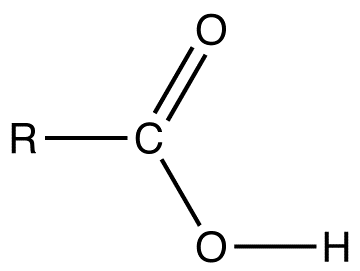
\includegraphics{carboxylic_acid.png}
\centering
\end{figure}

\section{Esters}
Esters have a pair of alkyl or aromatic groups attached to a carbonyl + linking
oxygen function.

Esters can be shown as \texttt{RCOOR}.

The reaction between a carboxylic acid and an alcohol produces an ester and
water.
This is an acid catalyzed equilibrium.

\begin{figure}[ht]
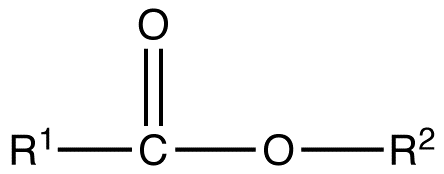
\includegraphics{ester.png}
\centering
\end{figure}

\section{Amides}
\subsection{Primary Amides}
Primary amides have an alkyl or aromatic group attached to an amino-carbonyl
function.

Primary amides can be shown as \texttt{RCONH2}.

\subsection{Secondary Amides}
Secondary amides have an alkyl or aryl group attached to the nitrogen:
\texttt{RCONHR}.

\subsection{Tertiary Amides}
Tertiary amides have two alkyl or aryl group attached to the nitrogen:
\texttt{RCONR2}.

\section{Amines}
\subsection{Primary amine}
Primary amines have an alkyl or aromatic group and two hydrogens attached to a
nitrogen atom.

Primary amines are basic functions that can be protonated to the corresponding
ammonium ion.
Primary amines are also nucleophilic.

Primary amines can be shown as \texttt{RNH2}.

\subsection{Secondary amine}
Secondary amines have a pair of alkyl or aromatic groups, and a hydrogen,
attached to a nitrogen atom.

Secondary amines are basic functions that can be protonated to the corresponding
ammonium ion.
Secondary amines are also nucleophilic.

Secondary amines can be shown as \texttt{R2NH}.

\subsection{Tertiary amine}
Tertiary amines have three alkyl or aromatic groups attached to a nitrogen atom.

Tertiary amines are basic functions that can be protonated to the corresponding
ammonium ion.
Tertiary amines are also nucleophilic.

Tertiary amines can be shown as \texttt{R3N}.

\section{Acid chlorides}
Acid chlorides, or acyl chlorides, have an alkyl (or aromatic) group attached to
a carbonyl function plus a labile (easily displaced) chlorine.

Acid chlorides highly reactive entities are highly susceptible to attack by
nucleophiles.
Acid chlorides can be shown as \texttt{RCOCl}.

\section{Acid anhydrides}
Acid anhydrides are formed when water is removed from a carboxylic acid, hence
the name.

Acid anhydrides can be shown as \texttt{(RCO)2O}.

\begin{figure}[ht]
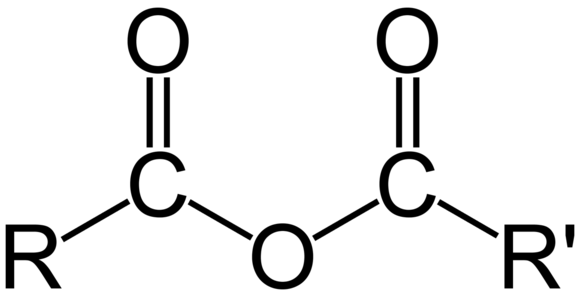
\includegraphics[scale=0.2]{carboxylic-acid-anhydride.png}
\centering
\end{figure}

\section{Nitriles}
Nitriles (or organo cyanides) have an alkyl (or aromatic) group attached to a
carbon-triple-bond-nitrogen function.

Nitriles can be shown as \texttt{RCN}.

Note that there is a nomenclature issue with nitriles/cyanides. If a compound is
named as the nitrile then the nitrile carbon is counted and included, but when
the compound is named as the cyanide it is not.

For instance, \texttt{CH3CH2CN} is called propane nitrile or ethyl cyanide
(cyanoethane).

\section{Carboxylate ion or salt}
Carboxylate ions are the conjugate bases of carboxylic acids, i.e. the
deprotonated carboxylic acid.

When the counter ion is included, the salt is being shown.

Salts can be shown as \texttt{RCOONa}.

\section{Amino Acids}
Amino acids, strictly alpha-amino acids, have carboxylic acid, amino function
and a hydrogen attached to a the same carbon atom.

There are 20 naturally occurring amino acids. All except glycine (R = H) are
chiral and only the L enantiomer is found in nature.

Amino acids can be shown as \texttt{R-CH(NH2)COOH}.

\begin{figure}[ht]
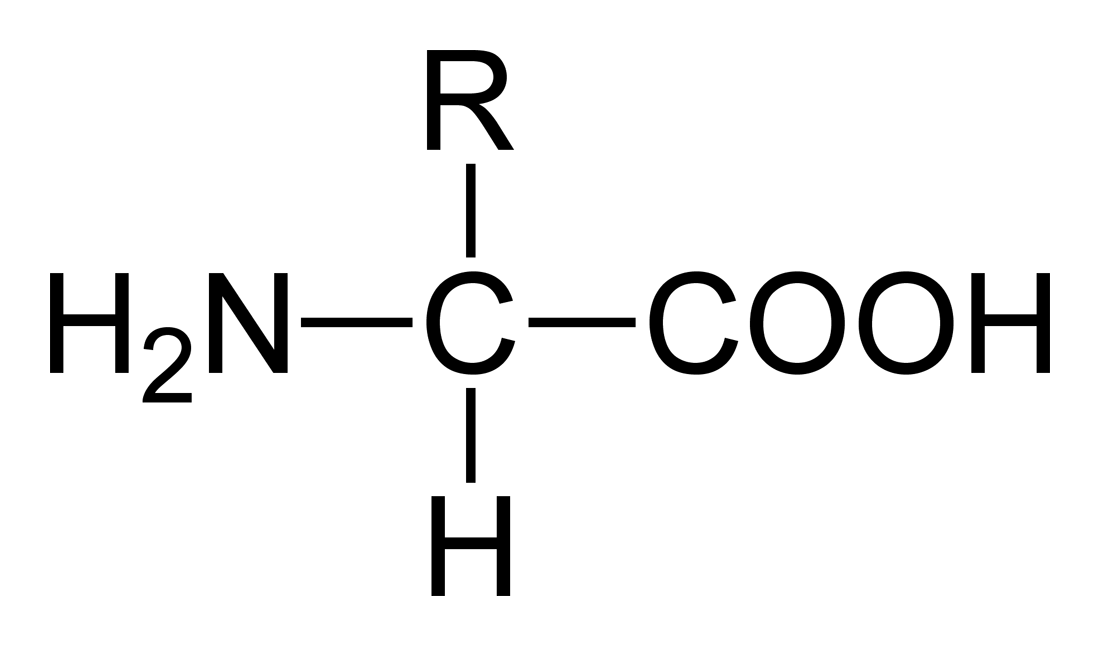
\includegraphics[scale=0.125]{alpha-amino-acid-flat.png}
\centering
\end{figure}

\section{Ethers}
Ethers have a pair of alkyl or aromatic groups attached to a linking oxygen
atom.

Ethers are surprisingly unreactive and are very useful as solvents for many many
(but not all) classes of reaction.

Ethers can be shown as \texttt{ROR}.

\section{Polymer}
Polymers consist of small monomer molecules that have reacted together so as to
form a large covalently bonded structure.

There are two general types of polymerisation: addition and condensation.

Linear chain polymers are generally thermoplastic, while three dimensional
network polymers are not. \textbf{Thermoplastic polymers} become pliable or
moldable above a specific temperature and solidify upon cooling, while
\textbf{thermosetting polymers} cure irreversibly. The cure may be induced by
heat, through a chemical reaction, or suitable irradiation. Thermoset materials
are usually liquid or malleable prior to curing and designed to be molded into
their final form, or used as adhesives. Once hardened a thermoset resin cannot
be reheated and melted to be shaped differently.

\part{Physics}

\chapter{Kinetics}
\[S = S_0 + V_0 t + \frac{a t^2}{2}\]
\[V_f^2 = V_i^2 + 2 a \Delta S\]

\chapter{Waves}
\[v = \lambda f\]

\section{Doppler Effect}
\[f = f_0 \left ( \frac{v + v_r}{v + v_s} \right )\]

where

\(v\) is the velocity of waves in the medium;

\(v_r\) is the velocity of the receiver relative to the medium; positive if the
receiver is moving towards the source (and negative in the other direction);

\(v_s\) is the velocity of the source relative to the medium; positive if the
source is moving away from the receiver (and negative in the other direction).

One can remember that the velocities are positive if the receiver is chasing
the source.

\section{Sound Intensity}
For a spherical sound wave, the intensity in the radial direction as a function
of distance \(r\) from the center of the sphere is given by

\[I(r) = \frac{P}{A(r)} = \frac{P}{4 \pi r^2}\]

\section{Pendulum}
The period of swing of a simple gravity pendulum depends on its length, the
local strength of gravity, and to a small extent on the maximum angle that the
pendulum swings away from vertical, called the amplitude. It is independent of
the mass of the bob. If the amplitude is limited to small swings, the period T
of a simple pendulum, the time taken for a complete cycle, is:
\[T \approx 2 \pi \sqrt{\frac{l}{g}}\]

\chapter{Optics}
\section{Mirrors and Lenses}
\textbf{Focal length}
\[\reciprocal{f} = \reciprocal{p} + \reciprocal{p'}\]
A positive value for \(p'\) indicates a real image, while a negative value
indicates a virtual image.

\(f\) is positive for concave mirrors and convex lenses, and negative for convex
mirrors and concave lenses.

\textbf{Magnification}
\[m = \frac{h'}{h} = - \frac{p'}{p} = \frac{f}{f - p}\]
\(h'\) is positive if the image is upright and negative if the image is upside
down. The value of \(h\) is always positive because the object is always
upright.

\chapter{Gases}
\[P = P_A + \rho g h\]
\[\tau = P \Delta V\]

\chapter{Electricity}
\[U = R i\]
\[P = i U\]
Resistance of a parallel association of resistors:
\[\reciprocal{R_{eq}} = \sum{\reciprocal{R_i}}\]

\section{Electric Force}
\[F_{el} = \frac{k Q q}{r^2}\]

\section{Transformers}
A transformer makes use of Faraday's law and the ferromagnetic properties of an
iron core to efficiently raise or lower alternating current (AC) voltages.
For an ideal transformer, the voltage ratio is equal to the turns ratio, and
power in equals power out.

\[\frac{V_1}{V_2} = \frac{N_1}{N_2}\]

\[P_{\text{in}} = P_{\text{out}}\]

\chapter{Electromagnetism}

\section{Magnetic Force}
\[F_{mag} = B q v = B i l\]

\section{Magnetic Fields}
\[B_{\text{wire}} = \frac{i \mu_0}{2 \pi r}\]
\[B_{\text{current loop}} = \frac{i \mu_0}{2 r}\]
\[B_{\text{solenoid}} = \frac{i \mu_0 N}{l}\]

where \(N\) is the number of coils and \(l\) is the length of the solenoid in
meters.

\section{Lenz's Law}
Lenz's law is a common way of understanding how electromagnetic circuits obey
Newton's third law and the conservation of energy.
\begin{quote}
If an induced current flows, its direction is always such that it will oppose
the change which produced it.
\end{quote}
Lenz's law is shown with the negative sign in Faraday's law of induction:
\[{E}=-\frac{\partial \Phi}{\partial t}\]

\chapter{Modern Physics}
\[E = hf = h\frac{c}{\lambda}\]

\section{Lorentz factor}
The Lorentz factor is the factor by which time, length, and relativistic mass
change for an object while that object is moving.
\[\gamma = \reciprocal{\sqrt{1 - \frac{v^2}{c^2}}}\]

\section{Superposition}
Superposition is a principle of quantum theory that describes a challenging
concept about the nature and behavior of matter and forces at the sub-atomic
level. The principle of superposition claims that while we do not know what the
state of any object is, it is actually in all possible states simultaneously,
as long as we don't look to check. It is the measurement itself that causes the
object to be limited to a single possibility. It can also be said that there is
no single outcome unless it is observed.

Superposition is well illustrated by \textbf{Thomas Young's double-slit
experiment}, developed in the early nineteenth century to prove that light
consisted of waves. Richard Feynman claimed that the essentials of quantum
mechanics could be grasped by an exploration of the implications of Young's
experiment.

In this experiment, a beam of light is aimed at a barrier with two vertical
slits.  The light passes through the slits and the resulting pattern is
recorded.  If one slit is covered, the pattern is what would be expected: a
single line of light, aligned with whichever slit is open. Intuitively, one
would expect that if both slits are open, the pattern of light will reflect
that fact: two lines of light, aligned with the slits.  However, what happens
is that the plate is entirely separated into multiple lines of lightness and
darkness in varying degrees.  What is being illustrated by this result is that
interference is taking place between the waves/particles going through the
slits, in what, seemingly, should be two non-crossing trajectories.

We would expect that if the beam of light particles or photons is slowed enough
to ensure that individual photons are hitting the plate, there could be no
interference and the pattern of light would be two lines of light, aligned with
the slits. In fact, however, the resulting pattern still indicates
interference, which means that, somehow, the single particles are interfering
with themselves. This seems impossible: we expect that a single photon will go
through one slit or the other, and will end up in one of two possible light
line areas. But that is not what happens. As Feynman concluded, each photon not
only goes through both slits, but simultaneously takes every possible
trajectory en route to the target.

In order to see how this might possibly occur, experiments have focused on
tracking the paths of individual photons. What happens in this case is that the
measurement in some way disrupts the photons' trajectories (in accordance with
the uncertainty principle), and somehow, the results of the experiment become
what would be predicted by classical physics: two bright lines on the
photographic plate, aligned with the slits in the barrier. Cease the attempt to
measure, however, and the pattern will again become multiple lines in varying
degrees of lightness and darkness. Each photon moves simultaneously in a
superposition of possible trajectories, and, furthermore, measurement of the
trajectory causes the superposition of states to collapse to a single position.

Text extracted from
\href{http://whatis.techtarget.com/definition/superposition}{WhatIs}.

\part{Mathematics}

\chapter{Significant figures}

\section{Definition}
The significant figures of a number are those digits that carry meaning
contributing to its precision. This includes all digits except all leading zeros
and trailing zeros when they are used to indicate the scale of the number.

\section{Calculations}
The result of addition and subtraction should have as many decimal places as the
term with less decimal places.

The result of multiplication and division should have as many significant
figures as the least precise term.

\section{Rounding}
If the first non-significant figure is a 5 not followed by any other digits or
followed only by zeros, rounding requires a tie-breaking rule.
\paragraph{Round half up} is the default rounding method implied in many
disciplines if not specified.
\paragraph{Round half to even} which rounds to the nearest even number.

\chapter{Set Theory}
\section{Power Set}
The power set \(P(S)\) is the set of all subsets of \(S\), including the empty
set and the set \(S\) itself.

It has \(2^n\) elements where \(n\) is the number of elements in \(S\).

\chapter{Linear Algebra}

\section{Row operations}
\begin{itemize}
\item{Replace one row by the sum of itself and a multiple of another row.}
\item{Interchange two rows.}
\item{Multiply all entries in a row by a nonzero constant.}
\end{itemize}

\section{Row equivalence}
Two matrices are \textbf{row equivalent} if, and only if, there is a sequence
of row operations that transform one matrix into another.
Row equivalence is indicated by a tilde (\(\sim\)) between matrices.
\section{Echelon form}
A matrix is in \textbf{echelon form} if it has the shape resulting from a
Gaussian
elimination.
The following are properties of the echelon matrix:
\begin{itemize}
\item{All nonzero rows are above any rows of all zeros.}
\item{The leading entry of a row is at least one column to the right of the
leading entry of the row above it.}
\end{itemize}
The following are properties of the \textbf{reduced echelon matrix}:
\begin{itemize}
\item{The leading entry in any nonzero row is 1.}
\item{Each leading 1 is the only nonzero in its column.}
\end{itemize}

\section{Row reducing algorithm}
The \textbf{forward phase} of the row reducing algorithm produces the row
echelon form.
The \textbf{backward phase} produces the unique reduced row echelon form.
Computer algorithms usually select as a pivot the entry in a column that has the
largest value.
This strategy, called partial pivoting, is used to reduce roundoff errors in the
calculations.
Computers do not perform the backward phase in order to find the reduced echelon
form, instead,
they perform back substitution.
The best strategy is to use the reduced echelon form only when solving a system
by hand.
A flop is one arithmetic operation (+, -, *, /) on two real floating point
numbers.
(Traditionally, + and - were not considered to be flops, but nowadays they are).

\section{Solution existence and uniqueness}
A solution exists if there are no invalid equations, such as \( 0 = 1 \). The
solution is unique if, and only if, there are no free variables.

\subsection{Existence and uniqueness theorem}
A system is consistent if, and only if, the rightmost column of the augmented
matrix is not a pivot column.
Stated differently, a matrix equation of the form \(A\mathbf{x} = \mathbf{b}\)
has a solution if, and only if, \(\mathbf{b}\) is a linear combination of the
columns of \(\mathbf{A}\), that is, if \(\mathbf{b} \in \mathrm{Span}
\{\mathbf{a}_1, \ldots, \mathbf{a}_n\}\).

\section{Parallelogram Rule for Addition}
If \(\mathbf{u}\) and \(\mathbf{v}\) in \(\mathbb{R}^2\)
are represented as points in the plane,
then \(\mathbf{u} + \mathbf{v}\) corresponds to the fourth vertex of the
parallelogram whose other vertices are \(\mathbf{0}\), \(\mathbf{u}\) and
\(\mathbf{v}\).

\section{Linear combinations}
Given vectors \(\mathbf{v}_1, \mathbf{v}_2, \ldots, \mathbf{v}_p\) in
\(\mathbb{R}^n\) and given scalars \(c_1, c_2, \ldots, c_p\) in \(\mathbb{R}\),
the vector \(\mathbf{y}\) defined by
\[ \mathbf{y} = c_1 \mathbf{v}_1 + \ldots + c_p \mathbf{v}_p \]
is called a \textbf{linear combination} of
\(\mathbf{v}_1, \ldots, \mathbf{v}_p\) with weights \(c_1, \ldots, c_p\).

\section{Span}
The set of all linear combinations of \(\mathbf{v}_1, \ldots, \mathbf{v}_p\) in
\(\mathbb{R}^n\) is called the \textbf{subset of}\(\mathbb{R}^n\) spanned (or
generated) by \(\mathbf{v}_1, \ldots, \mathbf{v}_p\) and is denoted by

\(\mathrm{Span}\{\mathbf{v}_1, \ldots, \mathbf{v}_p\}\). If a matrix \(A\) has a
pivot in every row, then \(\mathrm{Span} \{\mathbf{a}_1, \ldots, \mathbf{a}_n\}
= \mathbb{R}^m\).

\section{Matrix equation solution}
If \(A\) is a \(m \times n\) matrix, with columns \(\mathbf{a}_1, \ldots,
\mathbf{a}_n\) and \(\mathbf{b}\) is in \(\mathbb{R}^m\),
the matrix equation
\[ A\mathbf{x} = \mathbf{b} \]
has the same solution as the vector equation
\[ x_1\mathbf{a}_1 + \ldots + x_n\mathbf{a}_n = \mathbf{b} \]
which, in turn,
has the same solution as the system of linear equations whose
augmented matrix is
\[ [ \mathbf{a}_1 \ldots \mathbf{a}_n \mathbf{b} ] \]

\section{Solution sets of linear systems}
A system of linear equations is \textbf{homogeneous}
if it can be written in the form \( \mathbf{A x} = \mathbf{0} \).
All homogeneous systems have a \textbf{trivial solution} that is \(\mathbf{0}\).
If the system has at least one free variable, it has a nontrivial solution.

\begin{theorem*}
  Suppose that \( \mathbf{Ax} = \mathbf{b} \) is consistent for some given
  \(\mathbf{b}\), let \(\mathbf {p}\) be a solution. Then the solution set of
  \( \mathbf{Ax} = \mathbf{b} \) is the set of all vectors of the form
  \( \mathbf{w} = \mathbf{p} + \mathbf{v} \), where \( \mathbf{v} \) is any
  solution of the homogeneous equation \( \mathbf{Ax} = \mathbf{0} \).
\end{theorem*}

\section{Solution of a system in parametric form}
\begin{enumerate}
\item{Row reduce the augmented matrix to reduced row echelon form.}
\item{Express each basic variable in terms of any free variables.}
\item{Write \(\mathbf{x}\) as a vector whose entries depend on the free
variables.}
\item{Decompose \(\mathbf{x}\) into a linear combination of vectors.}
\end{enumerate}

\subsection*{Solved problem}
Write the general solution of \( 10 x_1 - 3 x_2 - 2 x_3 = 7\)
in parametric vector form.
\[ \left[ \begin{array}{cccc}
10 & -3 & -2 & 7 \end{array} \right] \sim
\left[ \begin{array}{cccc}
1 & -.3 & -.2 & .7 \end{array} \right] \]
    \[ x_1 = .7 + .3x_2 + .2x_3 \]
  \[ \mathbf{x} = \left[ \begin{array}{c} .7 \\ 0 \\ 0 \end{array} \right]
+ x_2 \left[ \begin{array}{c} .3 \\ 1 \\ 0 \end{array} \right]
+ x_3 \left[ \begin{array}{c} .2 \\ 0 \\ 1 \end{array} \right] \]

\section{Applications of Linear Systems}
In this section, it is shown how linear systems with multiple solutions can
arise naturally.
\subsection{Leontief model}
Also known as the Leontief ``production'' model.
If one knows the total output of a sector for a certain period of time and how
it is
divided among other sectors, then it is proven that
\begin{quote}
There exist equilibrium prices that can be assigned to the total outputs of the
various sectors in such a way that the income of each sector exactly balances
its
expenses.
\end{quote}

Suppose the following model is a decent representation of an economic.
\begin{center}
\begin{tabular}{| c c c | l |}
\hline
Coal & Electric & Steel & Purchased by \\
\hline
.0 & .4 & .6 & Coal \\
.6 & .1 & .2 & Electric \\
.4 & .5 & .2 & Steel \\
\hline
\end{tabular}
\end{center}

Then it is known that the equilibrium price of coal \(p_C = .4p_E + .6p_S\).
Therefore, \(p_C - .4p_E - .6p_S = 0\). Similar equations can be obtained from
the other two lines. At the end of the process, the linear system is

\[
\begin{bmatrix}
1   & -.4 & -.6 & 0 \\
-.6 &  .9 & -.2 & 0 \\
-.4 & -.5 &  .8 & 0
\end{bmatrix}
\]

By solving this system, it is known that

\[
p = \begin{bmatrix} p_C \\ p_E \\ p_S \end{bmatrix}
= \begin{bmatrix} .94 p_S \\ .85 p_S \\ p_S \end{bmatrix}
\]

Any (nonnegative) choice for \(p_S\) results in correct equilibrium prices.

\subsection{Balancing Chemical Equations}
Chemical equations describe the consumption of reactants and the formation
of products in chemical reactions.
Simple linear systems may be used to balance chemical reactions.
The burning of butanol is represented by:
\[
\left( x_1 \right) \text{C}_4\text{H}_{10}\text{O} +
\left( x_2 \right) \text{O}_2 \rightarrow
\left( x_3 \right) \text{CO}_2 +
\left( x_4 \right) \text{H}_2\text{O}
\]
In order to balance this reaction,
one must find the coefficients that make both sides have the same amount of
carbon,
hydrogen and oxygen.
This problem can be rewritten as:
\[
x_1 \begin{bmatrix} 4 \\ 10 \\  1\end{bmatrix} +
x_2 \begin{bmatrix} 0 \\  0 \\  2\end{bmatrix} +
x_3 \begin{bmatrix}-1 \\  0 \\ -2\end{bmatrix} +
x_4 \begin{bmatrix} 0 \\ -2 \\ -1\end{bmatrix} =
\begin{bmatrix}0 \\ 0 \\ 0\end{bmatrix}
\]
Row reduction of the corresponding augmented matrix gives us
\[
\textbf{p} = \begin{bmatrix}.2x_4 \\ 1.2x_4 \\ .8x_4 \\ x_4\end{bmatrix}
\]
The smallest selection of \(x_4\) that makes all coefficients integers is \(5\).
This makes
\[
  \text{C}_4\text{H}_{10}\text{O} +
6 \text{O}_2 \rightarrow
4 \text{CO}_2 +
5 \text{H}_2\text{O}
\]
a balanced chemical reaction.

\subsection{Network flow}
Systems of linear equations arise when scientists study the flow of something
through a network.
For instance, traffic engineers monitor the pattern of traffic flow in a grid of
city streets.
Electrical engineers calculate current flow through circuits.
And economists analyze the distribution of products from manufacturers to
consumers.
A network consists of a set of points (called junctions or nodes),
with lines or arcs called branches connecting some or all of the junctions.
The direction of flow in each branch is indicated,
and the flow amount (rate) is either shown or is denoted by a variable.
The basic assumption of network flow is that the total flow into the network
equals
the total flow out of the network and that the total flow into a junction equals
the total
flow out of the junction.
In a similar fashion, the flow at each junction is described by a linear
equation. The
problem of network analysis is to determine the flow in each branch when partial
information (such as the flow into and out of the network) is known.

\subsection{Solved exercises}
\subsubsection{Introduction}
This exercises are from the fourth edition of Linear Algebra and its
Applications.
\subsubsection{Leontief model}
\paragraph{1)}
An economy has four sectors: Agriculture, Manufacturing, Services, and
Transportation.
Agriculture sells 20\% of its output to Manufacturing, 30\% to Services, 30\% to
Transportation, and retains the rest.
Manufacturing sells 35\% of its output to Agriculture, 35\% to Services, 20\% to
Transportation, and retains the rest.
Services sells 10\% of its output to Agriculture, 20\% to Manufacturing, 20\% to
Transportation, and retains the rest.
Transportation sells 20\% of its output to Agriculture, 30\% to Manufacturing,
20\% to Services, and retains the rest.

\begin{enumerate}
\item Construct the exchange table for this economy.
\item Find a set of equilibrium prices for the economy if the value of
  Transportation is \(\$10.00\) per unit.
\item {The Services sector launches a successful ``eat farm fresh'' campaign,
       and increases its share of the output from the Agricultural sector to
40\%,
       whereas the share of Agricultural production going to Manufacturing falls
to 10\%.
       Construct the exchange table for this new economy.}
\item {Find a set of equilibrium prices for this new economy if the value of
    Transportation is still \(\$20.00\) per unit.
       What effect has the ``eat farm fresh'' campaign had on the equilibrium
prices for the sectors in this economy?}
\end{enumerate}

\subparagraph{Solution}

\begin{enumerate}
  \item {
  \[ \begin{bmatrix}
.2 & .35 & .1 & .2 \\
.2 &  .1 & .2 & .3 \\
.3 & .35 & .5 & .2 \\
.3 &  .2 & .2 & .3
      \end{bmatrix} \]}
  \item{\(p_A = 7.99\), \(p_M = 8.36\), \(p_S = 14.65\), and \(p_T = 10.00\).}
  \item {\[ \begin{bmatrix}
.2 & .35 & .1 & .2 \\
.1 &  .1 & .2 & .3 \\
.4 & .35 & .5 & .2 \\
.3 &  .2 & .2 & .3
            \end{bmatrix} \]}
  \item{\(p_A = 7.81\), \(p_M = 7.67\), \(p_S = 15.62\), and \(p_T = 10.00\).}
  \item{Therefore, the campaign has benefited Services.}
\end{enumerate}

\section{Matrices}
\subsection{Properties of the determinant}
\begin{enumerate}
  \item{\(\det(I)=1\).}
  \item{\(\det(A)=\det(A^{T})\).}
  \item{If \(B\) is \(A\) with a row multiplied by \(k\),
      then \(\det(B)=k\det(A)\).}
  \item{If \(B\) is \(A\) with two rows swapped, then \(\det(B)=-\det(A)\).}
  \item{If two or more rows of \(A\) are identical, then \(\det(A)=0\).}
  \item{If the elements above or below the diagonal of \(A\) are \(0\), then
      \(\det(A)=\prod_{i=1}^{m}{A_{i,i}}\).}
  \item{If the elements of \(A\), \(B\), and \(C\) are equal,
      except for one row of C that is equal to the sum of the two corresponding
      rows of \(A\) e \(B\), then
      \(\det{\left(C\right)}=\det{\left(A\right)}+\det{\left(B\right)}\).}
  \item{For square matrices \(A\) and \(B\) of equal size,
      \(\det{\left(AB\right)}=\det{\left(A\right)}\det{\left(B\right)}\).}
  \item{If \(B\) is \(A\) with one row multiplied by a nonzero constant added
      to a parallel row, then then \(\det(A)=\det(B)\).}
  \item{\(\det{\left(A^{-1}\right)}=\frac{1}{\det{\left(A\right)}}\).}
\end{enumerate}

\subsection{Inverse matrix}

\begin{proof}
The inverse matrix is unique.

Let \(B\) and \(C\) be the inverse matrices of \(A\).
\[B = BI = B(AC) = (BA)C = IC = C\]
\end{proof}

\subsubsection{Inverse matrix by Gauss-Jordan}
\[ \left[\mathrm{A} \mid \mathrm{I} \right] \rightarrow
\left[\mathrm{I} \mid \mathrm{A} ^ {-1} \right] \]

The adjoint matrix is the transposed of the cofactor matrix.
\[A^{-1} = \frac{\mathrm{adj}(A)}{\mathrm{D}} =
\frac{(\mathrm{cof}(A))^{T}}{\mathrm{D}}\]

\subsection{Singular matrix}
A square matrix that does not have a matrix inverse. A matrix is singular if,
and only if, its determinant is 0.


\chapter{Series}

\section{Arithmetic Series}
An arithmetic series is the sum of a sequence in which each term is computed
from the previous one by adding (or subtracting) a constant.
\[a_n = a_1 + (n-1)r\]
\[S_{p..q} = \frac{(q - p + 1)(a_q + a_p)}{2}\]
Note that this expression is just the product of the number of terms by the
average value.

\section{Geometric Series}
\[a_n = a_1 q^{(n-1)}\]
\[S_n = a_1 \frac{q^n - 1}{q-1}\]

\chapter{Complex numbers}

\section{Notation}
\[\cis \left ( \argument \right ) =  \cos \left ( \argument \right ) + i \sin
\left ( \argument \right )\]

\section{Formulas}
\[a + bi = r \left( \cos \left ( \argument \right ) + i \sin \left ( \argument
\right ) \right )
= r \cis \left ( \argument \right )\]
\[\conj{z} = a - bi = r \cis \left (- \argument \right)\]
\[r = \sqrt{a^2 + b^2}\]
\[\phi = \tan^{-1} \left ( \frac{b}{a} \right)\]

\[z_1 z_2 = r_1 r_2 \left ( \cis \left ( \phi_1 + \phi_2 \right ) \right )\]
\[\frac{z_1}{z_2} = \frac{r_1}{r_2} \left ( \cis \left ( \phi_1 - \phi_2 \right
) \right )\]
\[z^n = r^n \cis \left ( n \argument \right )\]
\[z^{\reciprocal{n}} = r^{\reciprocal{n}} \cis \left ( \frac{\argument + 2 \pi
k}{n} \right ), \quad
k : k \in \integers \text{ and } 0 \le k \le n - 1\]

Euler's Formula
\[e^{ix} = \cis \left ( x \right)\]

\chapter{Logarithms}

\paragraph{Logarithm.} The logarithm is the inverse operation to exponentiation.
The natural logarithm of \(t\) equals the integral of \(x^{-1}\) in respect to x
from \(1\) to \(t\).

\section{Definition}

\[y = \log_a x \iff a^y = x, \quad a > 0, a \ne 0\]
\[\log_a 0 = \begin{cases} -\infty, \quad a > 1 \\ +\infty, \quad a < 1
\end{cases}\]
\[\log x y = \log x + \log y\]
\[\log \frac{x}{y} = \log x - \log y\]
\[\log x^n = n \log x\]
\[\log_a b = \frac{\log_c b}{\log_c a} = \left ( \log_a c \right ) \left (
\log_c b \right )\]
\[\log a_b = \reciprocal{\log_b a}\]
\[e=\lim_{k\to\infty} \left ( 1 + \reciprocal{k} \right ) ^ k\]

\chapter{Statistics}

\section{Linear Relationship}
A linear relationship between \(y\) and \(x\) is denoted by:
\[\mu_{y | x} = \beta_0 + \beta_1 x + \epsilon\]
where
\begin{itemize}
  \item[\(\mu_{y | x}\)] is the true mean of y for a given value of x
  \item[\(\beta_0 + \beta_1 x\)] is a line
  \item[\(\epsilon\)] is a random error
\end{itemize}

The estimated relation line:
\[\hat y = \hat {\beta_0} + \hat {\beta_1} x\]

\section{Pythagorean means}
The three classical Pythagorean means are the arithmetic mean (A), the
geometric mean (G), and the harmonic mean (H). They are defined by:
\[A = \frac{\sum{x}}{n}\]
\[G = \left( \prod{x} \right) ^ \reciprocal{n}\]
\[H = \frac{n}{\sum{\reciprocal{x}}}\]

If all \(x\) are positive, the following relation holds
\[min \le H \le G \le A \le max\]

\section{Measures of statistical dispersion}
Variance
\[\sigma^2 = \sum \frac{\left ( k-\mean{x} \right ) ^ 2}{n}\]
Standard Deviation
\[\sigma = \sqrt{\sum \frac{\left ( k-\mean{x} \right ) ^ 2}{n}}\]

\section{Normal distribution}
The normal distribution is a common continuous probability distribution denoted
by \(N(\mu, \sigma)\). \(\mu\) is the mean of the distribution (and also its
median and mode) and \(\sigma\) is its standard deviation.

If \(\mu = 0\) and \(\sigma = 1\), the distribution is called the
\textbf{standard normal distribution}.

\chapter{Geometry}

\section{Trigonometry}

For a right triangle with sides a and b, hypotenuse c
\[\sin{\alpha} = \frac{a}{c}\]
\[\cos{\alpha} = \frac{b}{c}\]
\[\tan{\alpha} = \frac{a}{b}\]
\[\csc{\alpha} = \reciprocal{\sin{\alpha}} = \frac{c}{a}\]
\[\sec{\alpha} = \reciprocal{\cos{\alpha}} = \frac{c}{b}\]
\[\cot{\alpha} = \reciprocal{\tan{\alpha}} = \frac{b}{a}\]

Sums and differences of sines, cosines, and tangents
\[{\sin{\left( \alpha \pm \beta \right)} =
  \sin{\alpha}\cos{\beta} \pm \sin{\beta}\cos{\alpha}}\]
\[{\cos{\left( \alpha \pm \beta \right)} =
  \cos{\alpha}\cos{\beta} \mp \sin{\alpha}\sin{\beta}}\]
\[{\tan{\left( \alpha \pm \beta \right)} =
  \frac{\tan{\alpha} \pm \tan{\beta}}{1 \mp \tan{\alpha} \tan{\beta}}}\]

\section{Right Triangle}
For a right triangle with sides a and b, hypotenuse c, projections m and n (of
a and b, respectively), and height h,
the following expressions are true

\[a^2 = m c\]
\[b^2 = n c\]
\[h^2 = m n\]
\[a b = c h\]

\section{Equilateral Triangle}
\[h = \frac{a \sqrt{3}}{2}\]
\[r = \frac{a \sqrt{3}}{6}\]
\[R = \frac{a \sqrt{3}}{3}\]
\[A = \frac{a^2 \sqrt{3}}{4}\]

\section{All Triangles}
\[A = a b \sin \gamma \]
\[A = p r\]
\[A = \sqrt{p \left ( p - a \right ) \left ( p - b \right ) \left ( p - c
\right )}\]

where

\begin{itemize}
  \item[\(p\)] is the semiperimeter;
  \item[\(r\)] is the inradius (the radius of the inscribed circle).
\end{itemize}

\paragraph{Median.} In geometry, a median of a triangle is a line segment
joining a vertex to the midpoint of the opposing side. Every triangle has
exactly three medians, one from each vertex. In the case of isosceles and
equilateral triangles, a median bisects any angle at a vertex whose two adjacent
sides are equal in length.

\paragraph{Relation to center of mass.} Each median of a triangle passes through
the triangle's centroid, which is the center of mass of an object of uniform
density in the shape of the triangle. Thus the object would balance on the
intersection point of the medians.

\paragraph{Each median divides the area of the triangle in half.}

\section{Law of sines}
\[\frac{a}{\sin{A}} = \frac{b}{\sin{B}} = \frac{c}{\sin{C}} = 2R\]
where \(a\), \(b\), and \(c\) are the lengths of the sides of a triangle, and
\(A\), \(B\), and \(C\) are the opposite angles, and \(R\) is the radius of
the triangle's circumcircle.

\section{Law of cosines}
\[a^2 = b^2 + c^2 - 2bc\cos{A}\]

\section{Quadrilateral}
\[A = \frac{d_1 d_2 \sin{\phi}}{2}\]

where

\begin{itemize}
  \item[\(d\)] is a diagonal;
  \item[\(\phi\)] is the angle between the diagonals.
\end{itemize}

\section{Regular Hexagon}

\[r = m = \frac{l \sqrt{3}}{2}\]
\[A = pr = 3 l r = \frac{3 l^2 \sqrt{3}}{2}\]

\section{Circle}
\paragraph{Intersecting Chord Theorem.} When two chords intersect each
other inside a circle, the products of their segments are equal.
\[a_1 a_2 = b_1 b_2\]

\section{Ellipse}
In mathematics, an ellipse is a curve on a plane that surrounds two focal points
such that the sum of the distances to the two focal points is constant for every
point on the curve.

An ellipse with center \(C \left( x_0, y_0 \right)\) is represented by
\[\frac{\left(x - x_0\right)^2}{a^2}+\frac{\left(y - y_0\right)^2}{b^2}=1\]
or
\[\frac{\left(x - x_0\right)^2}{b^2}+\frac{\left(y - y_0\right)^2}{a^2}=1\]
\subsection{Focus}
The focal distance \(c\) is given by the Pythagorean theorem:

\[a^2=b^2+c^2\]

\subsection{Area}
The area of an ellipse is:

\[A = \pi a b\]

\subsection{Eccentricity}
The eccentricity of an ellipse, usually denoted by \(\epsilon\), is the ratio of
the distance between the two foci, to the length of the major axis:

\[\epsilon = \frac{2f}{2a} = \frac{f}{a}\]

\section{Pyramids}
\[V = \frac{bh}{3}\]

\chapter{Equations}
\section{Discriminant}
\[\Delta = b^2 - 4ac\]

\section{Vieta's formulas}
A polynomial \(P(x) = a_n x^n + a_{n-1} x^{n-1} + ... + a_0\), (with the
coefficients being real or complex numbers and \(a_n \neq 0\)) is known by the
fundamental theorem of algebra to have \(n\) (not necessarily distinct) complex
roots \(x_1, x_2, ..., x_n\).

Vieta's formulas relate the polynomial's coefficients \(a_k\) to signed sums
and products of its roots \(x_i\) as follows:

\[\sum_{1 \le i \le n} x_i = - \frac{a_{n-1}}{a_n}\]
\[\sum_{1 \le i_1 < i_2 \le n} x_{i_1} x_{i_2} = \frac{a_{n-2}}{a_n}\]
\[\sum_{1 \le i_1 < i_2 < i_3 \le n} x_{i_1} x_{i_2} x_{i_3} = -
\frac{a_{n-3}}{a_n}\]
\[\sum_{1 \le i_1 < i_2 < ... < i_k \le n} x_{i_1} x_{i_2} ... x_{i_k} = (-1)^k
\frac{a_{n-k}}{a_n}\]

\chapter{Calculus}
\section{Series for \(e\)}
%\[e^x = \frac{x^0}{0!} + \frac{x^1}{1!} + \frac{x^2}{2!} + \frac{x^3}{3!} + \ldots\]

\subsection{Intuition behind this series}
The following demonstration should help one understand why the abovementioned
series converges to \(e\).

\begin{align*}
    \frac{\dif}{\dif x} e^x
    &= \frac{\dif}{\dif x} \left( \frac{x^0}{0!} + \frac{x^1}{1!} + \frac{x^2}{2!} + \frac{x^3}{3!} + \ldots \right) \\
    &= \frac{0 x^{-1}}{0!} + \frac{1 x^0}{1!} + \frac{2 x^1}{2!} + \frac{3 x^2}{3!} + \ldots \\
    &= \frac{x^0}{0!} + \frac{x^1}{1!} + \frac{x^2}{2!} + \ldots = e^x
\end{align*}

\section{Derivatives}
\[\frac{\dif}{\dif x} \sin x = \cos x\]
\[\frac{\dif}{\dif x} \cos x = -\sin x\]

\subsection{Identities}
\[\frac{\dif}{\dif x} \ln x = \reciprocal{x}\]
\textbf{Chain Rule}
\[\left\{f\left[g\left(x\right)\right]\right\}'
= f'\left[g\left(x\right)\right] g'\left(x\right)\]

\section{Series}
\subsection{Maclaurin series}
A Maclaurin series is a Taylor series expansion of a function about 0.

\[f\left(x\right) = f\left(0\right) + f'\left(0\right)x + f''\left(0\right)\frac{x^2}{2!} + f^{\left( 3 \right)}\left(0\right)\frac{x^3}{3!} + \ldots\]

\section{Indefinite Integrals}
\subsection{Reversed Chain Rule}
\paragraph{Examples}
\[\int \tan x \dif x = \int \frac{\sin{x}}{\cos{x}} \dif x\]
Letting \(f(x) = \cos x\),
\[\int \frac{\sin{x}}{\cos{x}} \dif x = - \int \frac{f'(x)}{f(x)} \dif x
= - \ln{f(x)} + C = - \ln{\cos x} + C = \]
Note that, in this case, \(g'(x) = x^{-1}\), and that the integral of the
reciprocal function is the natural logarithm function.

\subsection{Substitution}\label{substitution}
\paragraph{Examples}
\[\int \cos^3 x \dif x
= \int \left( 1 - \sin^2 x \right) \cos x \dif x
= \int \cos x \dif x - \int \sin^2 x \cos x \dif x\]
\[\int \cos x \dif x = \sin x + C\]
Let \(u = \sin x\), therefore \(\dif u = \cos x \dif x\).
\[\int \sin^2 x \cos x \dif x = \int u^2 \dif u = \frac{\sin^3 x}{3} + C\]
\[\int \cos x \dif x - \int \sin^2 x \cos x \dif x
= \sin x + \frac{\sin^3 x}{3} + C\]

\subsection{Trigonometric Substitutions}
Some integrals require the substitution of a variable by an expression. This is
the opposite of what is done in \ref{substitution}, on which an expression is
replaced by a variable.

The following table summarizes the most effective trigonometric substitutions
and their intervals. The interval restrictions are important to ensure that the
function which defines the substitution is one-to-one. \cite{stewart}

\begin{center}
    \begin{tabular}{ |c|c|c| }
        \hline
        Expression & Substitution & Interval \\
        \hline
        \(\sqrt{a^2 - x^2}\)
          & \(x = a\sin\theta\)
          & \(-\frac{\pi}{2} \le \theta \le \frac{\pi}{2}\) \\
        \(\sqrt{a^2 + x^2}\)
          & \(x = a\tan\theta\)
          & \(-\frac{\pi}{2} < \theta < \frac{\pi}{2}\) \\
        \(\sqrt{x^2 - a^2}\)
          & \(x = a\sec\theta\)
          & \(0 \le \theta < \frac{\pi}{2} \lor \pi \le \theta < \frac{3\pi}{2}\) \\
        \hline
    \end{tabular}
\end{center}

\paragraph{Example}
Find the area enclosed by an ellipse of the form
\[\frac{x^2}{a^2} + \frac{y^2}{b^2} = 1\]

Isolating \(y\) gives
\[y = \pm \frac{b}{a} \sqrt{a^2 - x^2}\]

The area of the ellipse on the first quadrant is given by
\[\int_{0}^{a} \frac{b}{a} \sqrt{a^2 - x^2} \dif x\]

This is one fourth of the total area of the ellipse, therefore
\[A = 4 \int_{0}^{a} \frac{b}{a} \sqrt{a^2 - x^2} \dif x\]

To solve the integral, let \(x = a\sin\theta\) and, consequently, \(\dif x = a
\cos \theta \dif \theta\). It is made simpler by changing the integration
limits. When \(x = 0\), \(\sin x = 0\), thus \(\theta = 0\). When \(x = a\),
\(\sin \theta = 1\), thus \(\theta = \pi / 2\).

\begin{align*}
    4 \int_{0}^{\frac{\pi}{2}} \frac{b}{a} \sqrt{a^2 - x^2} \dif x
    &= \frac{4b}{a} \int_{0}^{\frac{\pi}{2}} \sqrt{a^2 - a^2 \sin^2 \theta} a \cos \theta \dif \theta \\
    &= 4ab \int_{0}^{\frac{\pi}{2}} \sqrt{1 - \sin^2 \theta} \cos \theta \dif \theta \\
    &= 4ab \int_{0}^{\frac{\pi}{2}} \sqrt{\cos^2 \theta} \cos \theta \dif \theta \\
    &= 4ab \int_{0}^{\frac{\pi}{2}} \abs{\cos \theta} \cos \theta \dif \theta \\
    &= 4ab \int_{0}^{\frac{\pi}{2}} \cos^2 \theta \dif \theta \\
    &= 2ab \int_{0}^{\frac{\pi}{2}} 1 + \cos {2 \theta} \dif \theta \\
    &= 2ab \left[ \theta + \frac{1}{2} \sin {2 \theta} \right]_{0}^{\frac{\pi}{2}} \\
    &= 2ab \left(\frac{\pi}{2} + 0 - 0 - 0\right) \\
    &= \pi a b
\end{align*}

Which is the formula for the area of an ellipse. Furthermore, it is also the
formula for the area of a circle as a circle is an ellipse with \(a = b\).

\part{Computer Science}

\chapter{Number Representation}

\section{Fixed Point}
Fixed point is a form of representing real numbers with a fixed number of digits
after the radix point.

\subsection{Fixed Point Conversion Exercises}
\paragraph{Exercise} Convert \texttt{01101011} and \texttt{11001100} from fixed
point notation with four bits for the integral part and four bits for the
fractional part to decimal first using unsigned arithmetic and then using two's
complement.

\paragraph{Solution} Using unsigned arithmetic,
\[0110.1011_{2} = 4_{10} + 2_{10} + 0.5_{10} + 0.125_{10} + 0.0625_{10}
  = 6.6875_{10}\]
\[1100.1100_{2} = 8_{10} + 4_{10} + 0.5_{10} + 0.25_{10} = 12.75_{10}\]

Using two's complement,
\[0110.1011_{2} = 4_{10} + 2_{10} + 0.5_{10} + 0.125_{10} + 0.0625_{10}
 = 6.6875_{10}\]
\[1100.1100_{2} = \left( 8_{10} + 4_{10} \right) - 16_{10} + 0.5_{10}
 + 0.25_{10} = -3.25_{10}\]

\paragraph{Exercise} Evaluate the following expressions using 8-bit unsigned
fixed point arithmetic. The results should have 4 bits for the integral part and
4 bits for the fractional part. The results must be rounded if necessary.
Overflow and rounding must be indicated.

\begin{enumerate}
    \item \(0111.0110_{2} + 0010.0010_{2}\)
    \item \(1000.1001_{2} - 1001.1000_{2}\)
    \item \(11.101011_{2} + 001100.00_{2}\)
\end{enumerate}

\paragraph{Solution}

\begin{enumerate}
    \item \(0111.0110_{2} + 0010.0010_{2} = 1001.1000_{2}\)
    \item \(1000.1001_{2} - 1001.1000_{2} = 0010.0001_{2}\) \textbf{(overflow)}
    \item \(11.101011_{2} + 001100.00_{2} = 1111.1011_{2}\) \textbf{(rounding)}
\end{enumerate}

\section{Floating Point}
Floating point is a form of representing real numbers while supporting a
trade-off between range and precision.

All exact values a floating point may assume are of the form
\[\text{significand} \cdot \text{base}^\text{exponent}\]
where significand, base, and exponent are integers and base is greater than or
equal to two.

\subsection{Usage}
Albeit more computationally expensive than fixed point arithmetic, floating
point arithmetic is more commonly used in modern times. The main reasons for
this is that the same floating point format is suitable for representing a wider
range of values than its fixed point counterpart.

Supercomputers are often compared in terms of FLOPS. FLOPS stands for
floating-point operations per second. It is a more accurate measure of computer
performance for computers which make heavy usage of floating-poing
operations.

\subsection{IEEE 754}
The IEEE 754 is the IEEE standard for floating-point arithmetic. It is a
technical standard for floating-point computation established in 1985.

The value of a single precision IEEE-754 number is given by
\[\text{sign} \cdot \text{significand} \cdot 2^\text{exponent}\]

\subsubsection{IEEE 754 Number Formats}
The standard defines five number formats, two of which are in wide usage:
binary32 and binary64.

The binary32 format defines 32-bit floating point numbers in base 2. These are
also known as \textbf{single precision floating point numbers}. This format
delegates one bit to the sign, 8 bits to the exponent and the remaining 23 bits
to the significand.

The binary64 format defines 64-bit floating point numbers in base 2. These are
also known as \textbf{double precision floating point numbers}. This format
delegates one bit to the sign, 11 bits to the exponent and the remaining 52 bits
to the significand.

\subsubsection{IEEE 754 Conversion Algorithm}
In order to convert the decimal representation of a real number to an IEEE 754
number the following algorithm may be used.
\begin{enumerate}
\item Set the first bit if the number is negative.
\item Find the biggest power of two which is less than or equal to the absolute
    value of the number and express it in the exponent bits biased by 127.
\item Express the fractional part of the quotient between the number whose
    representation is of interest and the abovementioned power of two in the
    significand bits.
\end{enumerate}

\subsubsection{IEEE 754 Conversion Exercises}

\textbf{From Decimal to IEEE 754}

Convert -7 to a single-precision IEEE 754 floating point number.
\begin{enumerate}
\item It is negative, therefore the first bit is set.
\item The biggest power of two less than or equal to the absolute value is
    \(2^2 = 4\). Therefore, the exponent should be \(127 + 2 = 129\).
\item Determine the significand: \(7 \div 4 = 1.75\).
\item This results in \singleprecision{11000001011000000000000000000000}.
\end{enumerate}

Convert 255 to a single-precision IEEE 754 floating point number.
\begin{enumerate}
\item It is positive, therefore the first bit is unset.
\item The biggest power of two less than or equal to the absolute value is
    \(2^7 = 128\). Therefore, the exponent should be \(127 + 7 = 134\).
\item Determine the significand: \(255 \div 128 = 1.9921875\).
\item This results in \singleprecision{01000011011111110000000000000000}.
\end{enumerate}

\textbf{From IEEE 754 to Decimal}

An algorithm for these conversions is not described as it is much more obvious
than the one required for the conversion from decimals values to this floating
point format. One should be able to understand it from simply reading some of
the examples below.

Convert \singleprecision{01000110110000000000000000000000} from IEEE 754 single
precision floating point to a decimal number.
\begin{enumerate}
\item The first bit is unset, therefore it is positive.
\item The exponent is \(141 - 127 = 14\).
\item The significand is \(1 + 2^{-1} = 1.5\).
\item This results in \(1.5 \times 2^{14} = 1.5 \times 16384 = 24576\).
\end{enumerate}

Convert \singleprecision{11001011010100000000000011000000} from IEEE 754 single
precision floating point to a decimal number.
\begin{enumerate}
\item The first bit is set, therefore it is negative.
\item The exponent is \(150 - 127 = 23\).
\item The significand is \(1 + 2^{-1} + 2^{-3} + 2^{-16} + 2^{-17} =
    1.62502288818359375\).
\item This results in \(-1.62502288818359375 \times 2^{23} = 13,631,680\).
\end{enumerate}

\textbf{Finding Representation Limits}

\textit{Find the largest positive number that can be represented with a single
precision IEE 754 floating point number.}

Straightforwardly enough, this number has the largest possible significand and
the largest possible exponent of a normalized value.

Therefore, this number is \singleprecision{01111111011111111111111111111111},
which in decimal is

\begin{align}
    &\left(1 + \sum_{i=1}^{23} 2^{-i}\right) \times 2^{127} \nonumber \\
    &= \frac{16777215}{8388608} \times 2^{127} \nonumber \\
    &= 340282346638528859811704183484516925440 \label{largest-positive-32} \\
    &\approx 3.403 \times 10^{38} \nonumber
\end{align}

\textit{Find the second largest positive number that can be represented with a
single precision IEEE 754 floating point number.}

This number is easily derived from the largest positive number, which is
\ref{largest-positive-32}. To obtain the first number smaller than the current
number, one should subtract one from the significand bits. However, if the
significand is 1.0, one should make the significand the biggest possible value
it may assume and decrement the exponent\footnote{Take the two options as
alternatives to obtain a number smaller than the largest positive representable
number. Decrementing the exponent will produce a number equal to the product of
\(0.5\) and the largest positive number. However, decrementing the significand
bits would produce a number approximately equal to the product of
\(0.999999881\) and largest positive number. This clearly demonstrates that the
sought after number is found by decrementing the significant bits.}.

Therefore, the second largest positive number that can be represented with a
single precision IEEE 754 floating point number is

% Could have used align*, but let us keep using align in case we need labels in
% the future.
\begin{align}
    \left(1 + \sum_{i=1}^{22} 2^{-i}\right) \times 2^{127}
    &= \frac{8388607}{4194304} \times 2^{127} \nonumber \\
    &= 340282326356119256160033759537265639424 \nonumber \\
    &\approx 3.403 \times 10^{38} \nonumber
\end{align}

This also shows that the difference between the largest possible number and the
second largest possible number is approximately \(2.03 \times 10^{31}\).

\textit{Find the smallest positive number that can be represented with a single
precision IEE 754 floating point number.}

This number is the product of the smallest positive significand by the power of
the base raised to the smallest normalized exponent.

Namely, this number is \singleprecision{00000000100000000000000000000000}, whose
decimal representation is

\begin{align}
    2^{-126}
    &= \frac{1}{85070591730234615865843651857942052864}
    \label{smallest-positive-32} \\
    &\approx 1.175 \times 10^{-38} \nonumber
\end{align}

\textit{Find the second smallest positive number that can be represented with a
single precision IEE 754 floating point number.}

The opposite of what was done to find the second largest positive number may be
done to find the second smallest positive number. Therefore, the significand is
made \(1 + 2^{-23}\) and the exponent is left unchanged.

\begin{align}
    &\left(1 + 2^{-23}\right) \times 2^{-126} \nonumber \\
    &= \frac{8388609}{713623846352979940529142984724747568191373312} \nonumber
    \\ &\approx 1.175 \times 10^{-38} \nonumber
\end{align}

This also shows that the difference between the smallest possible number and the
second smallest possible number is approximately \(1.401 \times 10^{-45}\).

\textit{Find the sum of the following floating point numbers.}
\begin{description}
    \item \singleprecision{11000011010100000000000000000000}
    \item \singleprecision{01000110110000000000000000000000}
\end{description}

As the exponent of the positive number is greater, the result is positive.
Evaluating the addition is easier if the significands are aligned. In order to
achieve this, denormalize the negative value so that its exponent is also 14.
The \textbf{actual} significand then changes in the following way:

\begin{description}
    \item \FormatAsSignificandBits{1.1010000000}
    \item \FormatAsSignificandBits{0.0000001101}
\end{description}

Therefore, the operation on the significands is a simple binary subtraction.
Namely,

\[1.1000000000 - 0.0000001101 = 1.0111110011\]

This results in a normalized significand. Therefore, straightforwardly enough,
the complete result is \singleprecision{01000110101111100110000000000000}.

One might convert these numbers to decimal to better understand what is
happening. After doing so, it is found that the subtraction performed was
\(24576 - 208 = 24368\).

\chapter{Boolean Algebra}
\section{Boolean Expressions}
A way to convert a truth table into a Boolean expression is by writing an
expression that evaluates to true for each and every row that evaluates to true
and chain them together with the OR operator. This expression may later be
simplified through logic identities.

Any Boolean function can be expressed by an expression containing only AND and
NOT operations. For instance, \(A \lor B\) can be expressed as \(\lnot \left(
\left( \lnot A \right) \land \left( \lnot B \right) \right)\).

\subsection{de Morgan's Laws}
De Morgan's laws are a pair of transformation rules that are both valid rules of
inference. The rules allow the expression of conjunctions and disjunctions
purely in terms of each other via negation. In mathematical notation, the rules
state that
\[\lnot \left( A \land B \right) =
  \left( \lnot A \right) \lor \left( \lnot B \right)\]
and
\[\lnot \left( A \lor B \right) =
  \left( \lnot A \right) \land \left( \lnot B \right)\]
are valid equalities.

\chapter{Algorithms}

\section{Sorting}
\subsection{Selection Sort}
\paragraph{Algorithm Description.} Sort \(n\) numbers stored in array
\(\mathbf{A}\) by finding the smallest element of \(\mathbf{A}\) and exchanging
it with the element in \(\mathbf{A}[1]\). Then find the second smallest element
of \(\mathbf{A}\), and exchange it with \(\mathbf{A}[2]\). Continue in this
manner for the first \(n - 1\) elements of \(\mathbf{A}\).

\textbf{Implementation.}

\begin{lstlisting}
for i = 1 to A.length - 1
  // sI stands for smallestIndex
  sI = i
  for j = i + 1 to A.length
    if A[j] < A[sI]
      sI = j
  // swap (if necessary)
  if (sI != i)
    tmp = A[i]
    A[i] = A[sI]
    A[sI] = tmp
\end{lstlisting}

\textbf{Analysis.} The best-case for this algorithm is an already sorted data
array. The worst-case would be produced by a sorted array with the first element
moved to the last position and all the other elements moved one place to the
left. Note that the only thing that varies is the amount of swaps made, the
algorithm has \(\Theta(n^2)\) time-complexity even for sorted input.

\section{String matching}
\subsection{Rabin-Karp (1987)}
This algorithm speeds up equality testing by using a hash function.

If the hash of the substring from the text was recomputed at each iteration,
this would become an O(mn)-time algorithm, this problem is solved by reusing
the last computed hash in the evaluation of the new hash. Such a hash function
is called a \textbf{rolling hash}.

\textbf{Rabin Fingerprint}. This hash treats every substring as a number in a
base \(\alpha\), usually a large prime.

\begin{lstlisting}
  // A Rabin Fingerprint roll.
  hash -= first_char * a ^ (m - 1)
  hash *= a
  hash += new_last_char
\end{lstlisting}

This algorithm is slower than Knuth-Morris-Pratt and Boyer-Moore for single
pattern string searching because of its slow worst case behavior. However, it is
an algorithm of choice for multiple pattern search.

For instance, to find if any string of a large number of strings is in a text we
can create a variant of the Rabin-Karp algorithm that uses a set data structure
to check whether the hash of a substring belongs to a set of hash values of
patterns in constant time.

\chapter{Hardware}
\section{Hard Disks}
Any hard disk drive (HDD) can contain only four primary partitions. This
limitation may be circumvented with an extended partition, a special type of
primary partition that allows multiple logical partitions to be created within
it. An HDD may contain only one extended partition.

An HDD records data by magnetizing a thin film of ferromagnetic material on a
disk. Sequential changes in the direction of magnetization represent binary
data bits.

A typical HDD design consists of a spindle that holds flat circular disks, also
called platters, which hold the recorded data. The platters are made from a
non-magnetic material, usually aluminium alloy, glass, or ceramic, and are
coated with a shallow layer of magnetic material typically 10–20 nm in depth,
with an outer layer of carbon for protection.

The platters in contemporary HDDs are spun at speeds varying from 4,200 rpm in
energy-efficient portable devices, to 15,000 rpm for high-performance servers.
The first HDDs spun at 1,200 rpm and, for many years, 3,600 rpm was the norm.
Nowadays, the platters in most consumer-grade HDDs spin at either 5,400 rpm or
7,200 rpm.

Information is written to and read from a platter as it rotates past devices
called read-and-write heads that operate very close (often tens of nanometers)
over the magnetic surface. The read-and-write head is used to detect and modify
the magnetization of the material immediately under it.

\paragraph{Partial response maximum likelihood.} In computer data storage,
partial response maximum likelihood (PRML) is a method for converting the weak
analog signal from the head of a magnetic disk or tape drive into a digital
signal. PRML attempts to interpret correctly even small changes in the analog
signal, whereas peak detection relies on fixed thresholds. Because PRML can
correctly decode a weaker signal it \textbf{allows higher density recording}.

For example, PRML would read the magnetic flux density pattern 70, 60, 55, 60,
70 (where 60 is the baseline signal) as binary ``101'', and the same for 45, 40,
30, 40, 45 (baseline of 40) whereas peak detector would decode everything
above, say, 50 as high, and below 50 as low, so the first pattern would read
``111'' and the second as ``000''.

\chapter{Computer Networks}
\section{HTTP Status codes}
HTTP status codes convey the reulst of the attempts of the server to satisfy the
request
\begin{itemize}
 \item 1xx : informational
 \item 2xx : success
 \item 3xx : redirection
 \item 4xx : client error
 \item 5xx : server error
\end{itemize}

\chapter{Database theory}
Relational databases arose in the 80's. NoSQL databases are much more recent.

Transactions are all about atomic updates that either succeed or fail.

\textbf{The CAP theorem.} If a system has a network \textbf{partition}, it
cannot be fully \textbf{consistent} and fully \textbf{available}. In real-world
scenarios, usually the tradeoff is between consistency and response-time.

\section{Distributed systems}
Distributed systems may use sharding, in which only one copy of each aggregate
exists, or replication, on which multiples copied of the data are distributed.
\textbf{Replication improves availability and resilience}.

\section{Sample problems}
Two different users, interacting with two different servers that talk to the
same database retrieve data, edit it, and then write it back. If no precautions
are taken, this causes a write-write conflict (one update will overwrite the
other).

Solution A. Hold a transaction open until the update is complete. This makes it
impossible for two users to view the data at the same time. \textit{This is
impractical in most systems}.

Solution B. Make the final update a transaction so that the updates don't mix
together and use an \textbf{offline lock}. This is done by giving each record a
version stamp, if at the time of the update the version stamp has already been
updated (due to a database modification), you solve the conflict anyway you
want.

\section{Foreign Keys}
A foreign key is a field in a table that uniquely identifies an entry in another
table. The table that contains this field is the \textbf{child table} and the
referenced table is said to be the \textbf{parent table}.

\section{NoSQL}
The problem with relational databases was that a single logical structure in the
application ends up being split into several rows and tables. This is known as
\textbf{impedance mismatch}: the difficulties encountered when trying to map
an object into a table.

This led to \textbf{object databases}. They did not become popular because many
systems used relational databases for integration. This way, relational has
dominated into the 2000s. The change that happened to bring attention no NoSQL
was the popularization of the Internet. Some sites got a lot of traffic and
needed to scale. Using many simple computers, as Google and Facebook do is not
relational database friendly, as these databases are not easily distributed.

NoSQL (the term) was a hashtag someone came up with for a meetup Johan
Oskarsson proposed to discuss the problems with relational databases. Defining
NoSQL is almost impossible, but it is possible to list some common
characteristics of NoSQL databases:
\begin{itemize}
 \item They are non-relational.
 \item Most are cluster-friendly.
 \item Most are open source.
 \item They are related to 21st century web.
 \item They are schema-less.
\end{itemize}

There are four different data models NoSQL databases use.
The simplest one is \textbf{key-value}. It's like a persistent hashmap that can
store any kind of data.

There is also the \textbf{document model}. It is similar to JSON. Differently
from a key-value, this is much more transparent about what the data is.

Having no schema adds a lot of flexibility. But note that schema-less is not
accurate as most if not all documents have an \textit{implicit schema}. For
instance, all items may have \texttt{price} even if it is not required.

Most key-value databases allow you to store metadata about the values, what
makes them somewhat similar to document databases.

Document databases usually provide access by ID, what further blurries the line
between key-value and document databases.

There is also the \textbf{column family model}, which is slightly more complex.
In these databases, a row key maps to a set of column families.

These three types of NoSQL databases are also known as \textbf{aggregate
models}. They are better at clustering because each node gets a set of
aggregates that contain all the data a query needs and thus avoid the need of
building the result from small pieces obtained from different nodes.

If you need to slice data in several different ways, aggregate databases are not
a good idea.

The fourth and last type of NoSQL database is \textbf{graph databases}. These go
in the opposite direction of the other three, making the structure even less
rigid than a table. All four are schema-less and which one you use depends on
how do you work with your data.

If you use aggregates all the time, aggregate oriented databases are your best
bet. If you need to really break things up and jump around in a complex
structure, graph databases are the way to go. But in the end what works best for
you may be the good and old tabular structure provided by relational databases.

NoSQL databases ease development when there are natural aggregates and when
there is just too much data for a single server.
Aggregate-oriented databases are ACID within aggregates, concurrency issues show
up when a single transaction must change multiple documents.

\section{BASE}
Base is an alternative to ACID.
It stands for

\begin{enumerate}
  \item \textbf{B}asic \textbf{A}vailability
  \item \textbf{S}oft state
  \item \textbf{E}ventually consistent
\end{enumerate}

\chapter{Functional Programming}
In functional programming, functions are treated as data.

\printbibliography

\end{document}
